Shipyard \citep{shipyard} is a web-based user interface for docker.
In many ways the functionality of shipyard meets the requirements of \emph{rmt}, outlined in section \ref{sec:reqs}, as it has the ability to monitor containers and multiple hosts.
However, the application has little ``at-a-glance'' features relevant to \emph{rmt}.
For example, to view all hosts in the application, the user has to enter a separate menu, shown in figure \ref{fig:shipyardHosts}.
This page displays only the network information about the host, such as hostname and port, and no system resource information.
Given the limited resources available on the Raspberry Pi boards, resource monitoring is a crucial component of any monitoring tool to be used with the PiCloud, so Shipyard would not be an appropriate option for use with the PiCloud.

Some design features were noted however, and these are outlined in section \ref{sec:implUi}.

\begin{figure}[t]
	\centering
	\setlength\fboxsep{0pt}
	\setlength\fboxrule{0.5pt}
	\fbox{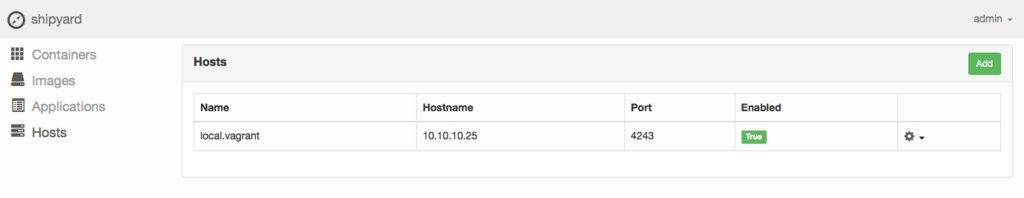
\includegraphics[width=0.8\textwidth]{shipyardHosts}}
	\caption{Hosts page in Shipyard}
	\label{fig:shipyardHosts}
\end{figure}
